%% bare_conf.tex
%% V1.4b
%% 2015/08/26
%% by Michael Shell
%% See:
%% http://www.michaelshell.org/
%% for current contact information.
%%
%% This is a skeleton file demonstrating the use of IEEEtran.cls
%% (requires IEEEtran.cls version 1.8b or later) with an IEEE
%% conference paper.
%%
%% Support sites:
%% http://www.michaelshell.org/tex/ieeetran/
%% http://www.ctan.org/pkg/ieeetran
%% and
%% http://www.ieee.org/

%%*************************************************************************
%% Legal Notice:
%% This code is offered as-is without any warranty either expressed or
%% implied; without even the implied warranty of MERCHANTABILITY or
%% FITNESS FOR A PARTICULAR PURPOSE! 
%% User assumes all risk.
%% In no event shall the IEEE or any contributor to this code be liable for
%% any damages or losses, including, but not limited to, incidental,
%% consequential, or any other damages, resulting from the use or misuse
%% of any information contained here.
%%
%% All comments are the opinions of their respective authors and are not
%% necessarily endorsed by the IEEE.
%%
%% This work is distributed under the LaTeX Project Public License (LPPL)
%% ( http://www.latex-project.org/ ) version 1.3, and may be freely used,
%% distributed and modified. A copy of the LPPL, version 1.3, is included
%% in the base LaTeX documentation of all distributions of LaTeX released
%% 2003/12/01 or later.
%% Retain all contribution notices and credits.
%% ** Modified files should be clearly indicated as such, including  **
%% ** renaming them and changing author support contact information. **
%%*************************************************************************


% *** Authors should verify (and, if needed, correct) their LaTeX system  ***
% *** with the testflow diagnostic prior to trusting their LaTeX platform ***
% *** with production work. The IEEE's font choices and paper sizes can   ***
% *** trigger bugs that do not appear when using other class files.       ***                          ***
% The testflow support page is at:
% http://www.michaelshell.org/tex/testflow/



\documentclass[conference]{IEEEtran}
% Some Computer Society conferences also require the compsoc mode option,
% but others use the standard conference format.
%
% If IEEEtran.cls has not been installed into the LaTeX system files,
% manually specify the path to it like:
% \documentclass[conference]{../sty/IEEEtran}





% Some very useful LaTeX packages include:
% (uncomment the ones you want to load)


% *** MISC UTILITY PACKAGES ***
%
%\usepackage{ifpdf}
% Heiko Oberdiek's ifpdf.sty is very useful if you need conditional
% compilation based on whether the output is pdf or dvi.
% usage:
% \ifpdf
%   % pdf code
% \else
%   % dvi code
% \fi
% The latest version of ifpdf.sty can be obtained from:
% http://www.ctan.org/pkg/ifpdf
% Also, note that IEEEtran.cls V1.7 and later provides a builtin
% \ifCLASSINFOpdf conditional that works the same way.
% When switching from latex to pdflatex and vice-versa, the compiler may
% have to be run twice to clear warning/error messages.






% *** CITATION PACKAGES ***
%
%\usepackage{cite}
% cite.sty was written by Donald Arseneau
% V1.6 and later of IEEEtran pre-defines the format of the cite.sty package
% \cite{} output to follow that of the IEEE. Loading the cite package will
% result in citation numbers being automatically sorted and properly
% "compressed/ranged". e.g., [1], [9], [2], [7], [5], [6] without using
% cite.sty will become [1], [2], [5]--[7], [9] using cite.sty. cite.sty's
% \cite will automatically add leading space, if needed. Use cite.sty's
% noadjust option (cite.sty V3.8 and later) if you want to turn this off
% such as if a citation ever needs to be enclosed in parenthesis.
% cite.sty is already installed on most LaTeX systems. Be sure and use
% version 5.0 (2009-03-20) and later if using hyperref.sty.
% The latest version can be obtained at:
% http://www.ctan.org/pkg/cite
% The documentation is contained in the cite.sty file itself.






% *** GRAPHICS RELATED PACKAGES ***
%
\ifCLASSINFOpdf
  % \usepackage[pdftex]{graphicx}
  % declare the path(s) where your graphic files are
  % \graphicspath{{../pdf/}{../jpeg/}}
  % and their extensions so you won't have to specify these with
  % every instance of \includegraphics
  % \DeclareGraphicsExtensions{.pdf,.jpeg,.png}
\else
  % or other class option (dvipsone, dvipdf, if not using dvips). graphicx
  % will default to the driver specified in the system graphics.cfg if no
  % driver is specified.
  % \usepackage[dvips]{graphicx}
  % declare the path(s) where your graphic files are
  % \graphicspath{{../eps/}}
  % and their extensions so you won't have to specify these with
  % every instance of \includegraphics
  % \DeclareGraphicsExtensions{.eps}
\fi
% graphicx was written by David Carlisle and Sebastian Rahtz. It is
% required if you want graphics, photos, etc. graphicx.sty is already
% installed on most LaTeX systems. The latest version and documentation
% can be obtained at: 
% http://www.ctan.org/pkg/graphicx
% Another good source of documentation is "Using Imported Graphics in
% LaTeX2e" by Keith Reckdahl which can be found at:
% http://www.ctan.org/pkg/epslatex
%
% latex, and pdflatex in dvi mode, support graphics in encapsulated
% postscript (.eps) format. pdflatex in pdf mode supports graphics
% in .pdf, .jpeg, .png and .mps (metapost) formats. Users should ensure
% that all non-photo figures use a vector format (.eps, .pdf, .mps) and
% not a bitmapped formats (.jpeg, .png). The IEEE frowns on bitmapped formats
% which can result in "jaggedy"/blurry rendering of lines and letters as
% well as large increases in file sizes.
%
% You can find documentation about the pdfTeX application at:
% http://www.tug.org/applications/pdftex





% *** MATH PACKAGES ***
%
%\usepackage{amsmath}
% A popular package from the American Mathematical Society that provides
% many useful and powerful commands for dealing with mathematics.
%
% Note that the amsmath package sets \interdisplaylinepenalty to 10000
% thus preventing page breaks from occurring within multiline equations. Use:
%\interdisplaylinepenalty=2500
% after loading amsmath to restore such page breaks as IEEEtran.cls normally
% does. amsmath.sty is already installed on most LaTeX systems. The latest
% version and documentation can be obtained at:
% http://www.ctan.org/pkg/amsmath





% *** SPECIALIZED LIST PACKAGES ***
%
%\usepackage{algorithmic}
% algorithmic.sty was written by Peter Williams and Rogerio Brito.
% This package provides an algorithmic environment fo describing algorithms.
% You can use the algorithmic environment in-text or within a figure
% environment to provide for a floating algorithm. Do NOT use the algorithm
% floating environment provided by algorithm.sty (by the same authors) or
% algorithm2e.sty (by Christophe Fiorio) as the IEEE does not use dedicated
% algorithm float types and packages that provide these will not provide
% correct IEEE style captions. The latest version and documentation of
% algorithmic.sty can be obtained at:
% http://www.ctan.org/pkg/algorithms
% Also of interest may be the (relatively newer and more customizable)
% algorithmicx.sty package by Szasz Janos:
% http://www.ctan.org/pkg/algorithmicx




% *** ALIGNMENT PACKAGES ***
%
%\usepackage{array}
% Frank Mittelbach's and David Carlisle's array.sty patches and improves
% the standard LaTeX2e array and tabular environments to provide better
% appearance and additional user controls. As the default LaTeX2e table
% generation code is lacking to the point of almost being broken with
% respect to the quality of the end results, all users are strongly
% advised to use an enhanced (at the very least that provided by array.sty)
% set of table tools. array.sty is already installed on most systems. The
% latest version and documentation can be obtained at:
% http://www.ctan.org/pkg/array


% IEEEtran contains the IEEEeqnarray family of commands that can be used to
% generate multiline equations as well as matrices, tables, etc., of high
% quality.




% *** SUBFIGURE PACKAGES ***
%\ifCLASSOPTIONcompsoc
%  \usepackage[caption=false,font=normalsize,labelfont=sf,textfont=sf]{subfig}
%\else
%  \usepackage[caption=false,font=footnotesize]{subfig}
%\fi
% subfig.sty, written by Steven Douglas Cochran, is the modern replacement
% for subfigure.sty, the latter of which is no longer maintained and is
% incompatible with some LaTeX packages including fixltx2e. However,
% subfig.sty requires and automatically loads Axel Sommerfeldt's caption.sty
% which will override IEEEtran.cls' handling of captions and this will result
% in non-IEEE style figure/table captions. To prevent this problem, be sure
% and invoke subfig.sty's "caption=false" package option (available since
% subfig.sty version 1.3, 2005/06/28) as this is will preserve IEEEtran.cls
% handling of captions.
% Note that the Computer Society format requires a larger sans serif font
% than the serif footnote size font used in traditional IEEE formatting
% and thus the need to invoke different subfig.sty package options depending
% on whether compsoc mode has been enabled.
%
% The latest version and documentation of subfig.sty can be obtained at:
% http://www.ctan.org/pkg/subfig




% *** FLOAT PACKAGES ***
%
%\usepackage{fixltx2e}
% fixltx2e, the successor to the earlier fix2col.sty, was written by
% Frank Mittelbach and David Carlisle. This package corrects a few problems
% in the LaTeX2e kernel, the most notable of which is that in current
% LaTeX2e releases, the ordering of single and double column floats is not
% guaranteed to be preserved. Thus, an unpatched LaTeX2e can allow a
% single column figure to be placed prior to an earlier double column
% figure.
% Be aware that LaTeX2e kernels dated 2015 and later have fixltx2e.sty's
% corrections already built into the system in which case a warning will
% be issued if an attempt is made to load fixltx2e.sty as it is no longer
% needed.
% The latest version and documentation can be found at:
% http://www.ctan.org/pkg/fixltx2e


%\usepackage{stfloats}
% stfloats.sty was written by Sigitas Tolusis. This package gives LaTeX2e
% the ability to do double column floats at the bottom of the page as well
% as the top. (e.g., "\begin{figure*}[!b]" is not normally possible in
% LaTeX2e). It also provides a command:
%\fnbelowfloat
% to enable the placement of footnotes below bottom floats (the standard
% LaTeX2e kernel puts them above bottom floats). This is an invasive package
% which rewrites many portions of the LaTeX2e float routines. It may not work
% with other packages that modify the LaTeX2e float routines. The latest
% version and documentation can be obtained at:
% http://www.ctan.org/pkg/stfloats
% Do not use the stfloats baselinefloat ability as the IEEE does not allow
% \baselineskip to stretch. Authors submitting work to the IEEE should note
% that the IEEE rarely uses double column equations and that authors should try
% to avoid such use. Do not be tempted to use the cuted.sty or midfloat.sty
% packages (also by Sigitas Tolusis) as the IEEE does not format its papers in
% such ways.
% Do not attempt to use stfloats with fixltx2e as they are incompatible.
% Instead, use Morten Hogholm'a dblfloatfix which combines the features
% of both fixltx2e and stfloats:
%
% \usepackage{dblfloatfix}
% The latest version can be found at:
% http://www.ctan.org/pkg/dblfloatfix




% *** PDF, URL AND HYPERLINK PACKAGES ***
%
%\usepackage{url}
% url.sty was written by Donald Arseneau. It provides better support for
% handling and breaking URLs. url.sty is already installed on most LaTeX
% systems. The latest version and documentation can be obtained at:
% http://www.ctan.org/pkg/url
% Basically, \url{my_url_here}.




% *** Do not adjust lengths that control margins, column widths, etc. ***
% *** Do not use packages that alter fonts (such as pslatex).         ***
% There should be no need to do such things with IEEEtran.cls V1.6 and later.
% (Unless specifically asked to do so by the journal or conference you plan
% to submit to, of course. )


% correct bad hyphenation here
\hyphenation{op-tical net-works semi-conduc-tor}


% Keywords command
\providecommand{\keywords}[1]
{
  \small	
  \textbf{\textit{Keywords---}} #1
}

\usepackage{hyperref}
\hypersetup{
    colorlinks=true,
    linkcolor=blue,
    filecolor=blue,      
    urlcolor=blue,
    pdftitle={PyGAD Paper},
    pdfpagemode=FullScreen}

\usepackage{graphicx}

\usepackage{xcolor}
\usepackage{xparse}
\usepackage{listings}
\NewDocumentCommand{\codeword}{v}{%
\texttt{\textcolor{blue}{#1}}%
}

% \usepackage{minted}
% \usemintedstyle{vs}

\usepackage{amsmath}

\lstset{language=C,keywordstyle={\bfseries \color{blue}}}

\usepackage{enumitem}

% Definindo novas cores
\definecolor{verde}{rgb}{0.25,0.5,0.35}
\definecolor{jpurple}{rgb}{0.5,0,0.35}
\definecolor{darkgreen}{rgb}{0.0, 0.2, 0.13}
%\definecolor{oldmauve}{rgb}{0.4, 0.19, 0.28}
% Configurando layout para mostrar codigos Java
\usepackage{listings}

\newcommand{\estiloPython}{
  \lstset{ %
    language=Python,                % the language of the code
    basicstyle=\footnotesize,       % the size of the fonts that are used for the code
    numbers=left,                   % where to put the line-numbers
    numberstyle=\tiny\color{gray},  % the style that is used for the line-numbers
    stepnumber=1,                   % the step between two line-numbers. If it's 1, each line
                                    % will be numbered
    linewidth=8.3cm,
    numbersep=5pt,                  % how far the line-numbers are from the code
    backgroundcolor=\color{white},  % choose the background color. You must add \usepackage{color}
    showspaces=false,               % show spaces adding particular underscores
    showstringspaces=false,         % underline spaces within strings
    showtabs=false,                 % show tabs within strings adding particular underscores
    frame=single,                   % adds a frame around the code
    rulecolor=\color{black},        % if not set, the frame-color may be changed on line-breaks within not-black text (e.g. commens (green here))
    tabsize=2,                      % sets default tabsize to 2 spaces
    captionpos=b,                   % sets the caption-position to bottom
    breaklines=true,                % sets automatic line breaking
    breakatwhitespace=false,        % sets if automatic breaks should only happen at whitespace
    title=\lstname,                 % show the filename of files included with \lstinputlisting;
                                    % also try caption instead of title
    keywordstyle=\color{blue},      % keyword style
    commentstyle=\color{darkgreen},   % comment style
    stringstyle=\color{red},      % string literal style
    escapeinside={\%*}{*)},         % if you want to add a comment within your code
    morekeywords={*,pygad,...}          % if you want to add more keywords to the set
}}

\title{Estilos para escrever Código Fonte em \LaTeX}
\author{Taciano}

\IEEEoverridecommandlockouts
\usepackage{tikz}
\usepackage{textcomp}
\usepackage{lipsum}
\usepackage{hyperref}

\newcommand\copyrighttext{
  \footnotesize \textcopyright 2021 Ahmed Fawzy Gad. Published at arXiv on June, 10 2021.
  Donation is open at PayPal (\href{https://www.paypal.com/paypalme/ahmedfgad}{paypal.me/ahmedfgad} or e-mail \href{mailto:ahmed.f.gad@gmail.com}{ahmed.f.gad@gmail.com}), OpenCollective (\href{https://opencollective.com/pygad}{opencollective.com/pygad}), and Interac e-Transfer (\href{mailto:ahmed.f.gad@gmail.com}{ahmed.f.gad@gmail.com}).}
\newcommand\copyrightnotice{
\begin{tikzpicture}[remember picture,overlay]
\node[anchor=south,yshift=10pt] at (current page.south) {\fbox{\parbox{\dimexpr\textwidth-\fboxsep-\fboxrule\relax}{\copyrighttext}}};
\end{tikzpicture}%
}

\begin{document}
%
% paper title
% Titles are generally capitalized except for words such as a, an, and, as,
% at, but, by, for, in, nor, of, on, or, the, to and up, which are usually
% not capitalized unless they are the first or last word of the title.
% Linebreaks \\ can be used within to get better formatting as desired.
% Do not put math or special symbols in the title.
\title{PyGAD: An Intuitive Genetic Algorithm Python Library}


% author names and affiliations
% use a multiple column layout for up to three different
% affiliations
\author{\IEEEauthorblockN{Ahmed Fawzy Gad}
\IEEEauthorblockA{School of Electrical Engineering and Computer Science\\
University of Ottawa\\
Ottawa, ON, Canada\\
\href{mailto:agad069@uottawa.ca}{agad069@uottawa.ca}}}




% use for special paper notices
%\IEEEspecialpapernotice{(Invited Paper)}




% make the title area
\maketitle

\copyrightnotice

% As a general rule, do not put math, special symbols or citations
% in the abstract
\begin{abstract}
This paper introduces PyGAD, an open-source easy-to-use Python library for building the genetic algorithm. PyGAD supports a wide range of parameters to give the user control over everything in its life cycle. This includes, but is not limited to, population, gene value range, gene data type, parent selection, crossover, and mutation. PyGAD is designed as a general-purpose optimization library that allows the user to customize the fitness function. Its usage consists of 3 main steps: build the fitness function, create an instance of the pygad.GA class, and calling the pygad.GA.run() method. The library supports training deep learning models created either with PyGAD itself or with frameworks like Keras and PyTorch. Given its stable state, PyGAD is also in active development to respond to the user's requested features and enhancement received on GitHub \href{https://github.com/ahmedfgad/GeneticAlgorithmPython}{github.com/ahmedfgad/GeneticAlgorithmPython}. PyGAD comes with documentation \href{https://pygad.readthedocs.io}{pygad.readthedocs.io} for further details and examples.
\end{abstract}

\keywords{genetic algorithm, evolutionary algorithm, optimization, deep learning, Python, NumPy, Keras, PyTorch}

% no keywords


% For peer review papers, you can put extra information on the cover
% page as needed:
% \ifCLASSOPTIONpeerreview
% \begin{center} \bfseries EDICS Category: 3-BBND \end{center}
% \fi
%
% For peerreview papers, this IEEEtran command inserts a page break and
% creates the second title. It will be ignored for other modes.
\IEEEpeerreviewmaketitle



\section{Introduction}
Nature has inspired computer scientists to create algorithms for solving computational problems. These naturally-inspired algorithms are called evolutionary algorithms (EAs) \cite{SimonEA} where the initial solution (or individual) to a given problem is evolved across multiple iterations aiming to increase its quality. The EAs can be categorized by different factors like the number of solutions used. Some EAs evolve a single initial solution (e.g. hill-climbing) and others evolve a population of solutions (e.g. particle swarm or genetic algorithm).

The genetic algorithm (GA) a biologically-inspired EA that solves optimization problems inspired by Darwin's theory ``survival of the fittest'' \cite{SimonEA, GadGA}. Originally, the GA was not designed for being a computational algorithm rather understanding how natural selection happens. Later, it becomes one of the most popular computational EAs.

The core concepts of the GA are derived from the natural solution. There are several organisms called population. The members of the population may have the ability to mate and reproduce new organisms. Because the good organisms can produce better offspring, then the good members of the population are selected for mating and others die. When 2 good organisms mate, their offspring will likely be better specially when some new, hopefully, better, changes are introduced. These concepts form the core of the GA in computer science.

The GA steps are explained in Figure \ref{fig:gasteps} \cite{GadGA}. The first step creates an initial population of solutions for the problems. These solutions are not the best for the problem and thus evolved. The evolution starts by selecting the fittest solutions as parents based on a maximization fitness function. Each pair of parents mate to produce one or more children. Each child shares genes from its 2 parents using the crossover operation. 

To go beyond the parents' capabilities, the mutation is introduced to make some changes to the children. Due to the randomness in these changes, some children may be fitter or worse than their parents. By mating the best parents and producing more children, a better solution is likely found after each generation. Either the offspring only or combined with the parents form the next generation's population. The process is repeated for a limited number of generations or until a satisfactory solution is found where no further optimization is necessary. 

% https://www.overleaf.com/learn/latex/Errors/%60!h'_float_specifier_changed_to_%60!ht'
\begin{figure}[t]
    \centering
    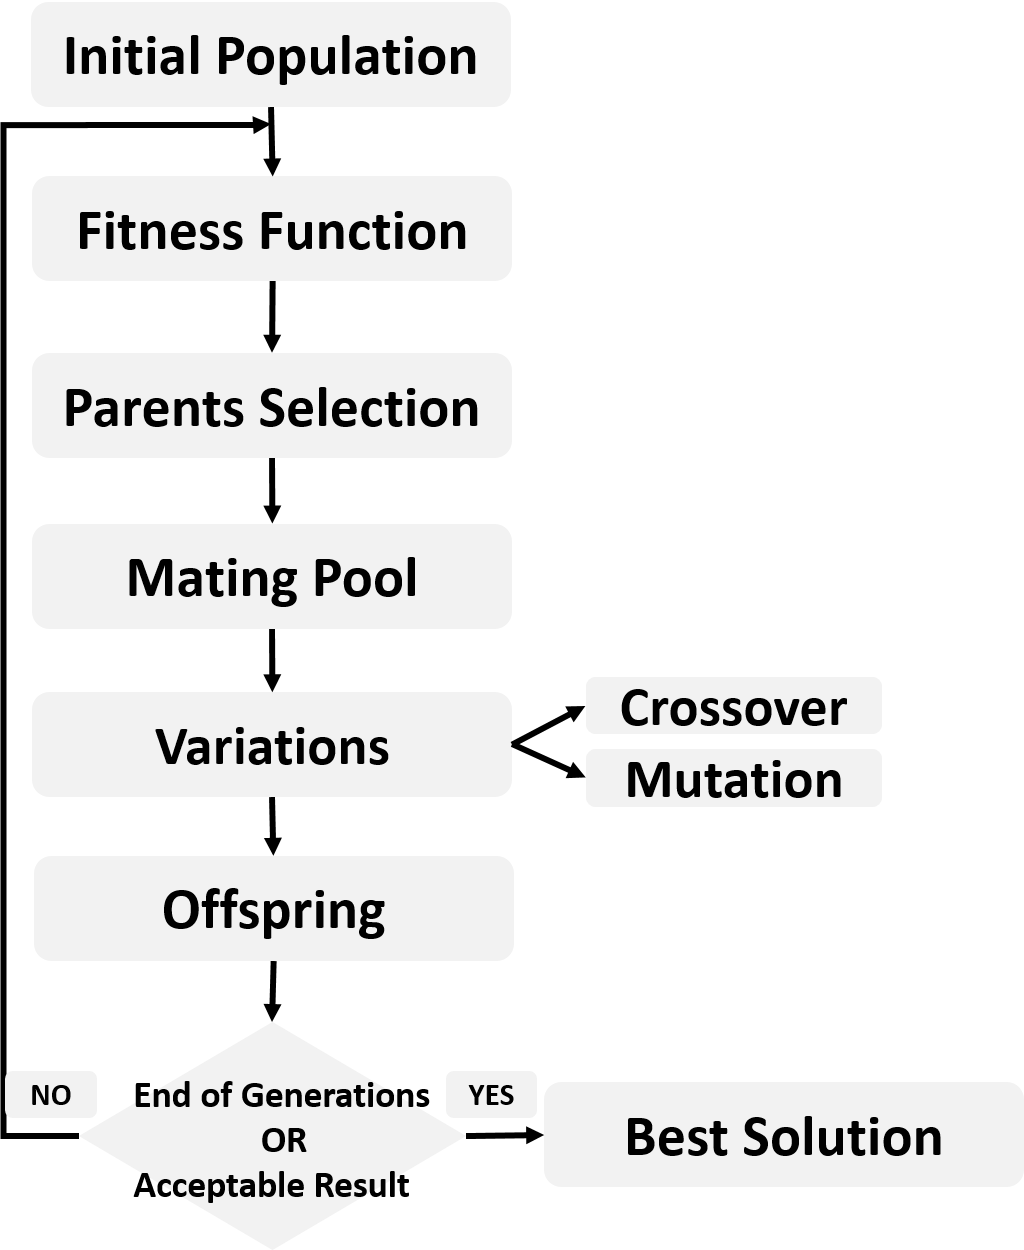
\includegraphics[width=8.7cm]{GASteps.png}
    \caption{Flowchart of the genetic algorithm.}
    \label{fig:gasteps}
\end{figure}

There are many parameters to tune in to make the GA fits the problem. For experimentation, it is essential to use an easy tool for building the genetic algorithm. 

This paper introduces PyGAD, an open-source intuitive Python library for optimization using the genetic algorithm. PyGAD was released in April 2020 and has over 185K installations at the time of writing this paper. The library supports single-objective optimization with a wide range of parameters to customize the GA for different types of problems in an easy-to-use way with less effort. PyGAD has a lifecycle to trace how everything is working from population creation until finding the best solution. The lifecycle can also be customized to help researchers alter its sequence, enable or disable some operations, make modifications, or introduce new operators. PyGAD works with both decimal and binary representations. The genes can be of \texttt{int}, \texttt{float}, or any supported \texttt{NumPy} numeric data types (\texttt{int}/\texttt{uint}/\texttt{float}). Given the advantages of the GA over the gradient-based optimizers, PyGAD supports training Keras and PyTorch models.

The paper is organized so that section \ref{relatedwork} covers the related work, section \ref{proposedlibrary} extensively introduces PyGAD and briefly compares PyGAD with DEAP and LEAP, and finally, section \ref{conclusion} draws conclusions. Appendix \ref{AppendixA} lists some resources to know more about PyGAD and Appendix \ref{AppendixB} lists the GitHub links of some projects built with PyGAD.

\section{Related Work}
\label{relatedwork}

There are already existing Python libraries for building the genetic algorithm. Some examples include:

\begin{enumerate}[label=\Alph*]
  \item \href{https://deap.readthedocs.io}{DEAP (Distributed Evolutionary Algorithms in Python)} \ref{deap}
  \item \href{http://pyevolve.sourceforge.net}{Pyevolve} \ref{pyevolve}
  \item \href{https://github.com/danielwilczak101/EasyGA}{EasyGA} \ref{easyga}
  \item \href{https://leap-gmu.readthedocs.io/en/latest}{LEAP (Library for Evolutionary Algorithms in Python)} \ref{leap}
\end{enumerate}

This section gives an overview of these libraries by explaining their objectives and limitations.

\subsection{DEAP}
\label{deap}
\href{https://deap.readthedocs.io}{DEAP (Distributed Evolutionary Algorithms in Python)} \cite{DEAP} is considered one of the most common Python libraries for optimization using the genetic algorithm based on the number of installations, GitHub issues, and stars (4.2K). One of the reasons is being one of the first libraries about EAs which was published in 2012. DEAP supports other algorithms than GA like non-dominated sorting genetic algorithm II (NSGA-II), particle swarm optimization (PSO), and evolution strategy (ES). Its latest release at Python Package Index (PyPI) is 1.3.1 released on Jan 2020.

DEAP uses 2 main structures which are \texttt{creator} and \texttt{toolbox}. The \texttt{creator} module is used for creating data types like fitness, individual, and population. These data types are empty and filled using the \texttt{toolbox} module. Given the special structure of DEAP, the user would take some time until understanding getting familiar. It needs more than a beginner's level in Python.

One problem about DEAP is being not user-friendly as the user has to do some efforts for each optimization problem. For example, the user has to write extra code for creating the population and filling it with appropriate values. The motivation for that is to enable the user to create custom data types that are not supported. But this boilerplate code unnecessarily increases the length of the Python script and makes it uncomfortable for users to write and understand more syntax about DEAP. Sometimes, the scripts are hard to read.

Moreover, the users have to create a main function in which everything is grouped in an evolutionary loop. The loop in this user-defined function should is where the user needs to follow the GA pipeline by 1) calculating the fitness function, 2) selecting the parents, 3) applying crossover and mutation, 4) and repeating that for several generations. This is not the best interface for users who try to focus on the experiments and save time on the other stuff. Writing the evolutionary loop makes the library non-friendly.

Even if the library supports some ready-to-use algorithms that save time building the main function, each algorithm does a specific task and is limited in its features. With the few parameters each algorithm accepts, there is little customization possible. Examples of these algorithms are \texttt{eaSimple}, \texttt{eaMuPlusLambda}, and \texttt{varOr}.

The library leaves much stuff to be built by the end-user which makes the user feel lost between the modules, classes, and functions needed to customize the library to solve a problem. For example, building a population of mixed data types requires the user to:

\begin{enumerate}
  \item Register a data type for each gene.
  \item Register an individual that combines those gene data types.
  \item Register a population that uses that individual.
  \item Build the population
\end{enumerate}

There is no way to restrict the gene values to a set of sparse discrete values. This is necessary for some problems where the gene value may not fall within a regular range. To select which genes to mutate, DEAP only supports the mutation probability. There is no way to specify the exact number of genes to be mutated. 

DEAP only supports the traditional mutation operators where all solutions, regardless of their fitness value, are given equal mutation probability. This would distort the high-quality solutions.

Another major drawback of DEAP is the lack of means of visualizing the results after the evolution completes \cite{DEAPReview}. The users have to manually create their plots to summarize the results.

\subsection{Pyevolve}
\label{pyevolve}
\href{http://pyevolve.sourceforge.net}{Pyevolve} is another pure Python library for building the genetic algorithm \cite{Pyevolve}. Even that it is published in 2009, it is less popular than DEAP and this is based on the total number of installations (50K for all the time), GitHub stars (301), and citations. It also has a limited community compared to DEAP. 

Its scripts start by creating the fitness function, preparing the chromosome, setting some parameters like which operators to use, create an instance of the \texttt{GSimpleGA} class and then call the \texttt{evolve()} method to start the evolution.

Like DEAP, this library has boilerplate code for configurations that makes its scripts unnecessarily longer even for simple problems. The supported mutation operators apply mutation equally to all solutions independent of their fitness value.

Even that Pyevolve is easier than DEAP, but it is limited in its features. It supports some predefined data types for the genes like integer and real. To create new data types, then more details about some classes in the library are needed like \texttt{GenomeBase.GenomeBase} which may be problematic for some users.

A comparison between DEAP and Pyevolve shows that the number of code lines needed to solve the OneMax problem is 59 for DEAP and 378 for Pyevolve \cite{DEAP}. Given the simplicity of the problem, Pyevolve needed too many lines.

This library is no longer maintained as the latest version was released at the end of 2014 and the most recent commit on its GitHub project was at the end of 2015.


\subsection{EasyGA}
\label{easyga}
The \href{https://github.com/danielwilczak101/EasyGA}{EasyGA} library allows only defining a continuous range for the gene values. If the range has some exclusions or if the gene values do not follow a range at all, then there is no way to define the gene values. Moreover, the user has to build the solutions manually without given a simple interface. Commonly, users would like to focus more on the algorithm itself and save time building additional modules specially if they are not involved in Python.

This library has a limited number of operators for crossover, mutation, and parent selection. Given the 

The EasyGA library supports a random mutation operation that applies mutation over any solution in the population, including parents, and is not restricted to the new offspring. It randomly selects the solutions to mutate. This is against the nature of the GA as only random changes could be introduced to the offspring, not the parents.

The users have to know about decorators, at some stage, to build their operators. While writing the paper, the GitHub project of EasyGA has only 22 stars.

\subsection{LEAP}
\label{leap}
\href{https://leap-gmu.readthedocs.io/en/latest}{LEAP (Library for Evolutionary Algorithms in Python)} is another recent Python library published in 2020 for EAs that supports the genetic algorithm \cite{LEAP}. This library has 3 core classes which are \texttt{Individual}, \texttt{Decoder}, and \texttt{Problem}. The decoder is responsible for converting the genes from one form to another to calculate the fitness value for each individual given the current problem. 

According to the examples posted by the developers, the decoder is usually set to \texttt{IdentityDecoder()} which means the gene is translated to itself. This is a design issue in the library. Maybe this feature is helpful in some specific problems but the library uses it as something essential for all types of problems.  It is better to work directly on the genes without having to decode them to another form or leave that decoding part to the fitness function. 

Even it is published in July 2020, the library has many missing features as mentioned in its documentation. One of these missing features is the mixed data representation in the individual. There is no lifecycle in LEAP to help trace what is happening in each generation.

Even if one of the objectives of LEAP is to make it simpler than the other libraries, the user still has to write the evolution loop. This results in more lines to solve a problem. Moreover, the user has to take care of calling a function that increases the generations counter by calling the \texttt{util.inc\_generation()} function. Avoiding to call it causes an infinite evolution loop. This would be a problem for users with less experience. 

Creating and managing the evolution loop is against another objective of LEAP to make it suitable for all types of software users (users who solve problems with existing tools).  

This library is not popular as it has a total of 3.4K installations since publication in addition to just 39 starts in the GitHub project. 

\section{Proposed PyGAD Library}
\label{proposedlibrary}

\href{https://pygad.readthedocs.io}{PyGAD} is an open-source Python library for optimization using the genetic algorithm. It is published in April 2020 at PyPI (\href{https://pypi.org/project/pygad}{pypi.org/project/pygad}). Its GitHub project has over 525 stars (\href{https://github.com/ahmedfgad/GeneticAlgorithmPython}{github.com/ahmedfgad/GeneticAlgorithmPython}). With over 185K installations over 1 year, PyGAD is the most rising library compared to the other libraries. 

The name PyGAD has 3 parts:
\begin{enumerate}
  \item \textbf{\textit{Py}} which means it is a \textit{Python} library. This is a common naming convention for Python libraries.
  \item \textbf{\textit{GA}} stands for \textit{genetic algorithm}.
  \item \textbf{\textit{D}} for \textit{decimal} because the library was originally supporting only decimal genetic algorithm. Now, it supports both decimal and binary genetic algorithm.
\end{enumerate}

This section gives an overview of \href{https://pygad.readthedocs.io}{PyGAD} \ref{pygadoverview}, discusses the steps of its usage \ref{pygadusage}, its lifecycle \ref{pygadlifecycle}, and main features in PyGAD \ref{pygadmainfeatures}. 

\subsection{PyGAD Overview}
\label{pygadoverview}

PyGAD is an intuitive library for optimization using the genetic algorithm. It is designed with 2 main objectives:
\begin{enumerate}
    \item Making everything as simple as possible for the users with the least knowledge.
    \item Giving the user control over everything possible.
\end{enumerate}

The simplicity comes from using descriptive names for the classes, methods, attributes, and parameters. This is in addition to making things straightforward to build the genetic algorithm and specify a wide range of easy-to-understand configuration parameters. There are fewer classes, methods, or functions to call to solve a problem compared to the other libraries. 

The users do not have to build the evolution loop in any situation as PyGAD supports an elastic lifecycle that can be altered. This includes, but is not limited to, enabling or disabling the mutation or crossover operators and overriding them to build new operators for research purposes.

The 7 modules included in PyGAD are:
\begin{enumerate}
    \item \texttt{pygad.pygad}: It is the main module which builds everything in the genetic algorithm. This module is implicitly imported when the library itself is imported.
    \item \texttt{pygad.nn}: Builds fully-connected neural networks (FCNNs) from scratch using only NumPy.
    \item \texttt{pygad.gann}: Uses the \texttt{pygad} module to train networks build using the \texttt{nn} module.
    \item \texttt{pygad.cnn}: Similar to the \texttt{nn} module but builds convolutional neural networks (CNNs).
    \item \texttt{pygad.gacnn}: Similar to the \texttt{gann} module but trains CNNs.
    \item \texttt{pygad.kerasga}: Trains Keras models using the \texttt{pygad} module.
    \item \texttt{pygad.torchga}: Trains PyTorch models using the \texttt{pygad} module.
\end{enumerate}

Given that the \texttt{pygad.pygad} is the most critical module in the library, it is given the most attention.

PyGAD has detailed documentation that covers all of its features with examples. Moreover, the source code of various projects built using PyGAD is explained in tutorials. A list of some of these tutorials is available in Appendix \ref{AppendixA}.

PyGAD gained popularity in the last months and some of its English articles and tutorials are translated to different languages like \href{https://pygad.readthedocs.io/en/latest/Footer.html#korean}{Korean}, \href{https://pygad.readthedocs.io/en/latest/Footer.html#turkish}{Turkish}, \href{https://pygad.readthedocs.io/en/latest/Footer.html#hungarian}{Hungarian}, \href{https://pygad.readthedocs.io/en/latest/Footer.html#chinese}{Chinese}, and \href{https://pygad.readthedocs.io/en/latest/Footer.html#russian}{Russian}. A list of such translated articles and tutorials is found in the \href{https://pygad.readthedocs.io/en/latest/Footer.html#pygad-in-other-languages}{PyGAD in Other Languages} section of the documentation.

The documentation of PyGAD has a section called \href{https://pygad.readthedocs.io/en/latest/Footer.html#release-history}{Release History} to summarize the changes and additions in each release.

Appendix \ref{AppendixA} has extra reading resources about PyGAD. Appendix \ref{AppendixB} lists some projects built with PyGAD.

\subsection{PyGAD Usage}
\label{pygadusage}

There are 3 core steps to use PyGAD:
\begin{enumerate}
    \item Build the fitness function.
    \item Instantiate the \texttt{pygad.GA} class with the appropriate configuration parameters.
    \item Call the \texttt{run()} method to start the evolution.
\end{enumerate}

For the following equation with 3 inputs, we can use PyGAD to find the values of $w_1$, $w_2$, and $w_3$ that satisfy equation:
\begin{gather*}
    Y = w_1X_1 + w_3X_3 + w_3X_3 \\
    Where \: Y=44, \; X_1=4, \; X_2=-2, \; and \; X_3=3.5
\end{gather*}

A basic PyGAD example that solves this problem is given in Listing \ref{lst:pygadexample}. Line \ref{line:importpygad} imports the library. This import statement implicitly imports the \texttt{pygad} module. The \texttt{NumPy} library is also imported in Line \ref{line:importnumpy} because it is used in the fitness function.

Line \ref{line:equationin} creates a Python list to hold the 3 inputs and line \ref{line:equationout} holds the output.

The fitness function in PyGAD is a regular Python function that accepts 2 parameters:
\begin{enumerate}
    \item The solution evolved by the genetic algorithm as a 1D vector. The function should return a single numeric value representing the fitness of this solution.
    \item The index of the solution within the population.
\end{enumerate}

The length of the solution in this example is 3, one value for each weight in the equation. The fitness function must be a maximization function (the higher the fitness value the better the solution).

The fitness function is defined from line \ref{line:fitnessfunctionstart} to line \ref{line:fitnessfunctionend} in Listing \ref{lst:pygadexample}. The function calculates the sum of products between each value in the solution and its corresponding input. The absolute difference is calculated between the sum and the output. 

Returning the absolute difference makes it a minimization function. This is why the result is returned as $1.0/abs$. A tiny value of $0.000001$ is added to the denominator to avoid diving by zero.

A new instance of the \texttt{pygad.GA} class is created in line \ref{line:pygadgainstance}. All configuration parameters are grouped in the \texttt{pygad.GA} class's constructor. With the available IDE's, the user can easily check the names of all available parameters. This way the user does not have to memorize the names of functions or classes compared to the other libraries. 

There are 5 required parameters that must be specified for each problem:
\begin{enumerate}
    \item \texttt{num\_generations}: The number of generations/iterations.
    \item \texttt{sol\_per\_pop}: The number of solutions/chromosomes/individuals in the population (i.e. population size).
    \item \texttt{num\_parents\_mating}: The number of solutions to be selected from the population as parents for mating and producing the offspring.
    \item \texttt{num\_genes}: The number of genes in each solution.
    \item \texttt{fitness\_func}: The fitness function.
\end{enumerate}

These are the minimum parameters to use PyGAD. Note that the names of the parameters are self-describing. The documentation has information about the classes, parameters, attributes, methods, and functions in all PyGAD modules. \hfill \break

\begin{scriptsize}
\estiloPython
\begin{minipage}{\linewidth}
\begin{lstlisting}[caption={PyGAD example.}, label=lst:pygadexample, escapechar=|]
import pygad |\label{line:importpygad}|
import numpy |\label{line:importnumpy}|

equation_inputs = [4, -2, 3.5] |\label{line:equationin}|
Y = 44 |\label{line:equationout}|

def fitness_func(solution, solution_idx): |\label{line:fitnessfunctionstart}|
    out = numpy.sum(solution * equation_inputs)
    fitness = 1.0/(numpy.abs(out - Y)+0.000001)
    return fitness |\label{line:fitnessfunctionend}|

ga_instance = pygad.GA(num_generations=100, |\label{line:pygadgainstance}|
                       sol_per_pop=10,
                       num_parents_mating=5,
                       num_genes=3,
                       fitness_func=fitness_func)

ga_instance.run() |\label{line:runga}|
\end{lstlisting}
\end{minipage}
\end{scriptsize}

In Listing \ref{lst:pygadexample}, a population of size 10 is evolved through 100 generations. Out of the population, 5 solutions are selected for mating. Each solution has 3 genes where the fitness value is calculated using the Python function named \texttt{fitness\_func}. 

The instances of the \texttt{pygad.GA} class has a method called \texttt{run()} which runs the genetic algorithm to start evolving the initial population according to the selected parameters. This is the minimal code for optimizing this problem using PyGAD.

Once the \texttt{run()} method completes, additional methods can be called to find information about the solution found by PyGAD. Two of these methods are:
\begin{enumerate}
    \item \texttt{best\_solution()}: Returns the following information about the best solution found by PyGAD:
    \begin{enumerate}
        \item The parameters of the best solution (e.g. the 3 weights for the problem solved in Listing \ref{lst:pygadexample}.
        \item The fitness value of the best solution.
        \item The index of this solution in its population.
    \end{enumerate}
    \item \texttt{plot\_result()}: Creates a plot showing how the fitness value evolves by each generation. This method returns the figure in case the user would like to save it.
\end{enumerate}

These 2 methods are called in Listing \ref{lst:pygadexampleplot}. Figure \ref{fig:pygadexample_plot} shows that the best solution is found after 31 generations only with a fitness value of 182.698. The best solution's parameters can be plugged into the equation to return the predicted value. \hfill \break

\begin{scriptsize}
\estiloPython
\begin{minipage}{\linewidth}
\begin{lstlisting}[caption={Evolution results.}, label=lst:pygadexampleplot, escapechar=|]
solution, solution_fitness, solution_idx = ga_instance.best_solution()
fig = ga_instance.plot_result()
\end{lstlisting}
\end{minipage}
\end{scriptsize}

For the OneMax optimization problem, it is solved with PyGAD in just 15 lines of code compared to 45 for DEAP and 34 for LEAP.

For 3 different runs with 100 generations each, the average time for PyGAD is 0.14 seconds compared to 0.65 for DEAP and 0.052 for LEAP. The trouble with LEAP is that the optimal solution was not found even after 1,000 generations. The maximum number of ones did not even reach $90/100$ after tens of trials with the code published by the developer at GitHub. 

\begin{figure}[t]
    \centering
    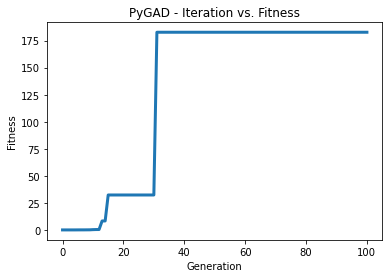
\includegraphics[width=8.7cm]{pygadexample_plot}
    \caption{Evolution of the fitness value for 100 generations.}
    \label{fig:pygadexample_plot}
\end{figure}

\subsection{PyGAD Lifecycle}
\label{pygadlifecycle}

PyGAD has a lifecycle that helps to user to keep track and control all different stages of the evolution process. Figure \ref{fig:pygad_lifecycle} shows the PyGAD lifecycle. Note that the side blocks refer to operations done between one state and another.

The passed parameters to the \texttt{pygad.GA} class's constructor are validated. Then, instance attributes are initialized according to the passed parameters. Some of these attributes include \texttt{population} which is a NumPy array holding all solutions in the population.

Once an instance of the \texttt{pygad.GA} class is created successfully, then it is time to start the lifecycle of PyGAD by calling the \texttt{run()} method. For the 7 states in PyGAD lifecycle, the following 7 callback functions exist:
\begin{enumerate}
    \item \texttt{on\_start()}: Called once after the \texttt{run()} method is called.
    \item \texttt{on\_fitness()}: Called after calculating the population fitness in each generation.
    \item \texttt{on\_parents()}: Called in each generation after the parents are selected.
    \item \texttt{on\_crossover()}: For each generation, it is called after applying the crossover operation.
    \item \texttt{on\_mutation()}: For each generation, it is called after applying the mutation operation.
    \item \texttt{on\_generation()}: Called at the end of each generation.
    \item \texttt{on\_stop()}: Called once after the \texttt{run()} method stops.
\end{enumerate}

The user can assign a Python function, with the appropriate parameters, to any of these callback functions. By doing this, the user can track and control everything from the start to the end of the evolution. This includes, but is not limited to, getting information about the population, fitness, selected parents, crossover or mutation results, and the best solution yet found. The user can also do some pre-processing or post-processing tasks in the \texttt{on\_start()} and \texttt{on\_stop()} functions, respectively. 

For research purposes and supporting an operator that is not supported by PyGAD, the user can define custom crossover and mutation operators in the callback functions. 

The \texttt{on\_generation()} callback function can be used to add some conditions and alter the execution. For example, returning the string "stop" immediately stops the \texttt{run()} method earlier before completing all generations.

\begin{figure}[t]
    \centering
    \includegraphics[width=8.7cm]{pygad_lifecycle}
    \caption{PyGAD lifecycle.}
    \label{fig:pygad_lifecycle}
\end{figure}

\subsection{PyGAD Features}
\label{pygadmainfeatures}

The previous sections should have covered some features of PyGAD. This section highlights the main features supported by PyGAD that make it distinctive compared to the other libraries. For more details, check its documentation \href{https://pygad.readthedocs.io}{pygad.readthedocs.io}.

\begin{enumerate}
  \item PyGAD is very intuitive to use. Its steps are self-explanatory and easy to follow in a user-friendly way. With just 3 simple steps, PyGAD can optimize different types of problems.
  \item All parameters are grouped in the constructor of the \texttt{pygad.GA} class. This helps the user to be focused and not distracted. 
  \item A user-defined gene value space, either for all genes at once or for each gene, can be created using the \texttt{gene\_space} parameter. This is helpful even if the gene's values do not follow a certain pattern. If a gene has values enclosed within a given range, then the gene value can be randomly generated from a user-defined range.
  \item It is possible to control the gene data type, for all genes or each gene, using the \texttt{gene\_type} parameter. The supported data types are Python's \texttt{int} and \texttt{float} in addition to all \texttt{int}/\texttt{uint}/\texttt{float} types in the \texttt{NumPy} library.
  \item Using the \texttt{initial\_population} parameter, a user-defined initial population can be used as the start point. This helps to continue where the evolution stopped. PyGAD builds an initial population randomly if this parameter is not set.
  \item PyGAD has a lifecycle to keep track of everything. A call to a callback function can be triggered for each step in the lifecycle.
  \item The user can stop the evolution at any time. For example, returning the string ``stop'' from the \texttt{on\_generation()} callback function stops PyGAD at the current generation.
  \item It is easy to access the best solutions across all generations in addition to their fitness using the \texttt{best\_solutions} and \texttt{best\_solutions\_fitness} attributes, respectively.
  \item The crossover and mutation operations can be disabled by setting \texttt{crossover\_type} or \texttt{mutation\_type} to \texttt{None} and then plug a user-defined operation in the lifecycle.
  \item There are different ways to specify the number of genes to mutate. According to the user's preference, this can be specified as probability (\texttt{mutation\_probability}), percentage (\texttt{mutation\_percent\_genes}), or an explicit number of genes (\texttt{mutation\_num\_genes}).
  \item PyGAD supports adaptive mutation so that the user controls how mutation is applied based on the solution's fitness. For the high-quality solutions, low mutation probability/percentage/number is expected compared to low-quality solutions. This helps to maintain the quality of the good solutions in addition to increasing the quality of the bad solutions.
  \item The \texttt{mutation\_by\_replacement} \texttt{bool} parameter selects whether the mutation adds to or replaces the gene value.
  \item A \texttt{bool} parameter called \texttt{allow\_duplicate\_genes} helps to accept or reject duplicate values in the same chromosome. For this to work, there must be enough value space to guarantee unique genes' values.
  \item Ability to control the number of parents to keep in the next generation using the \texttt{keep\_parents} parameter. This helps to save 0 or more parents to keep the fitness curve increasing.
  \item The instance attributes in the \texttt{pygad.GA} class starting with \texttt{last\_generation\_} help to keep track of the outcomes of each generation.
  \item PyGAD supports training \href{https://keras.io}{Keras} and \href{https://pytorch.org}{PyTorch} models using the \texttt{pygad.kerasga} and \texttt{torchga} modules, respectively.
  \item PyGAD also has its own modules to build and train neural networks (\texttt{pygad.nn}, \texttt{pygad.gann}, \texttt{pygad.cnn}, and \texttt{pygad.gacnn}).
  \item The interface to use any PyGAD feature is very simple and does not require much knowledge about Python compared to the other libraries. The minimum level is to know how to create variables, how to define a Python function that accepts parameters and returns something, little about classes like creating instances in addition to accessing class/instance attributes.
  \item PyGAD has built-in support to visualize the results. For example, the \texttt{best\_solution()} method shows how the fitness changes by generation.
  \item There are many resources to help you get started with PyGAD. This includes documentation, blog posts, examples, projects, and a community over \href{https://github.com/ahmedfgad/GeneticAlgorithmPython}{GitHub}, \href{https://www.reddit.com/search/?q=PyGAD&sort=relevance}{reddit}, \href{https://stackoverflow.com/search?q=PyGAD}{StackOverflow},  \href{https://www.facebook.com/pygad}{Facebook}, and \href{https://twitter.com/PyGADLib}{Twitter}.
\end{enumerate}

\section{Conclusion}
\label{conclusion}

This paper proposed a new Python library called PyGAD for single-objective optimization using the genetic algorithm. PyGAD is an intuitive library that makes it easy to optimize problems in just 3 steps: fitness function creation, instantiating the \texttt{pygad.GA} class, and calling \texttt{run()} method. There is a wide range of parameters and attributes to have a high degree of customizing the genetic algorithm. This includes defining a space of values for each gene, customizing each gene's data type, training Keras and PyTorch models, rejecting duplicates, and more. PyGAD has a lifecycle to keep track of the evolution process from the beginning to the end. PyGAD supports a simpler interface for users with less experience with Python to solve problems with few lines of code and even faster than the other libraries. 


% An example of a floating figure using the graphicx package.
% Note that \label must occur AFTER (or within) \caption.
% For figures, \caption should occur after the \includegraphics.
% Note that IEEEtran v1.7 and later has special internal code that
% is designed to preserve the operation of \label within \caption
% even when the captionsoff option is in effect. However, because
% of issues like this, it may be the safest practice to put all your
% \label just after \caption rather than within \caption{}.
%
% Reminder: the "draftcls" or "draftclsnofoot", not "draft", class
% option should be used if it is desired that the figures are to be
% displayed while in draft mode.
%
%\begin{figure}[!t]
%\centering
%\includegraphics[width=2.5in]{myfigure}
% where an .eps filename suffix will be assumed under latex, 
% and a .pdf suffix will be assumed for pdflatex; or what has been declared
% via \DeclareGraphicsExtensions.
%\caption{Simulation results for the network.}
%\label{fig_sim}
%\end{figure}

% Note that the IEEE typically puts floats only at the top, even when this
% results in a large percentage of a column being occupied by floats.


% An example of a double column floating figure using two subfigures.
% (The subfig.sty package must be loaded for this to work.)
% The subfigure \label commands are set within each subfloat command,
% and the \label for the overall figure must come after \caption.
% \hfil is used as a separator to get equal spacing.
% Watch out that the combined width of all the subfigures on a 
% line do not exceed the text width or a line break will occur.
%
%\begin{figure*}[!t]
%\centering
%\subfloat[Case I]{\includegraphics[width=2.5in]{box}%
%\label{fig_first_case}}
%\hfil
%\subfloat[Case II]{\includegraphics[width=2.5in]{box}%
%\label{fig_second_case}}
%\caption{Simulation results for the network.}
%\label{fig_sim}
%\end{figure*}
%
% Note that often IEEE papers with subfigures do not employ subfigure
% captions (using the optional argument to \subfloat[]), but instead will
% reference/describe all of them (a), (b), etc., within the main caption.
% Be aware that for subfig.sty to generate the (a), (b), etc., subfigure
% labels, the optional argument to \subfloat must be present. If a
% subcaption is not desired, just leave its contents blank,
% e.g., \subfloat[].


% An example of a floating table. Note that, for IEEE style tables, the
% \caption command should come BEFORE the table and, given that table
% captions serve much like titles, are usually capitalized except for words
% such as a, an, and, as, at, but, by, for, in, nor, of, on, or, the, to
% and up, which are usually not capitalized unless they are the first or
% last word of the caption. Table text will default to \footnotesize as
% the IEEE normally uses this smaller font for tables.
% The \label must come after \caption as always.
%
%\begin{table}[!t]
%% increase table row spacing, adjust to taste
%\renewcommand{\arraystretch}{1.3}
% if using array.sty, it might be a good idea to tweak the value of
% \extrarowheight as needed to properly center the text within the cells
%\caption{An Example of a Table}
%\label{table_example}
%\centering
%% Some packages, such as MDW tools, offer better commands for making tables
%% than the plain LaTeX2e tabular which is used here.
%\begin{tabular}{|c||c|}
%\hline
%One & Two\\
%\hline
%Three & Four\\
%\hline
%\end{tabular}
%\end{table}


% Note that the IEEE does not put floats in the very first column
% - or typically anywhere on the first page for that matter. Also,
% in-text middle ("here") positioning is typically not used, but it
% is allowed and encouraged for Computer Society conferences (but
% not Computer Society journals). Most IEEE journals/conferences use
% top floats exclusively. 
% Note that, LaTeX2e, unlike IEEE journals/conferences, places
% footnotes above bottom floats. This can be corrected via the
% \fnbelowfloat command of the stfloats package.



% conference papers do not normally have an appendix


% use section* for acknowledgment
\section*{Acknowledgment}

I would like to thank everyone who used or showed interest in PyGAD. Some of those people who reported issues or suggested useful features are \href{https://github.com/tfarrag2000}{Tamer Farrag} (Assistant Professor, Misr Higher Institute for Engineering and Technology, Egypt), \href{https://www.linkedin.com/in/hamadakassem}{Hamada Kassem} (RA/TA, Faculty of Engineering, Alexandria University, Egypt), \underline{Curt McDowell},  \href{https://www.mpibpc.mpg.de/17254711/andrei-rozanski}{Andrei Rozanski} (PhD Bioinformatics Specialist, Max Planck Institute for Biophysical Chemistry, Germany), \href{https://www.researchgate.net/profile/Marios-Giouvanakis}{Marios Giouvanakis} (PhD candidate in Electrical \& Computer Engineer, Aristotle University of Thessaloniki, Greece), \href{https://www.linkedin.com/in/l\%C3\%A1szl\%C3\%B3-fazekas-2429a912}{László Fazekas} (CTO Senior Software Developer at Pressenger Ltd, Hungary), and special thanks to \href{https://www.linkedin.com/in/rainer-matthias-engel-5ba47a9}{Rainer Engel} (Imaging Artist and Pipeline Developer, Germany) for his generous suggestions and time offered in inspecting PyGAD. 

% trigger a \newpage just before the given reference
% number - used to balance the columns on the last page
% adjust value as needed - may need to be readjusted if
% the document is modified later
%\IEEEtriggeratref{8}
% The "triggered" command can be changed if desired:
%\IEEEtriggercmd{\enlargethispage{-5in}}

% references section

% can use a bibliography generated by BibTeX as a .bbl file
% BibTeX documentation can be easily obtained at:
% http://mirror.ctan.org/biblio/bibtex/contrib/doc/
% The IEEEtran BibTeX style support page is at:
% http://www.michaelshell.org/tex/ieeetran/bibtex/
%\bibliographystyle{IEEEtran}
% argument is your BibTeX string definitions and bibliography database(s)
%\bibliography{IEEEabrv,../bib/paper}
%
% <OR> manually copy in the resultant .bbl file
% set second argument of \begin to the number of references
% (used to reserve space for the reference number labels box)
\begin{thebibliography}{1}

\bibitem{SimonEA}
Simon, Dan. \emph{Evolutionary optimization algorithms}. John Wiley \& Sons, 2013.

\bibitem{GadGA}
Gad, Ahmed Fawzy. Practical computer vision applications using deep learning with CNNs. Apress, 2018.
% H.~Kopka and P.~W. Daly, \emph{A Guide to \LaTeX}, 3rd~ed.\hskip 1em plus
%   0.5em minus 0.4em\relax Harlow, England: Addison-Wesley, 1999.

\bibitem{DEAP}
Fortin, Félix-Antoine, et al. "DEAP: Evolutionary algorithms made easy." The Journal of Machine Learning Research 13.1 (2012): 2171-2175.

\bibitem{DEAPReview}
Kim, Jinhan, and Shin Yoo. "Software review: Deap (distributed evolutionary algorithm in python) library." Genetic Programming and Evolvable Machines 20.1 (2019): 139-142.

\bibitem{Pyevolve}
Perone, Christian S. "Pyevolve: a Python open-source framework for genetic algorithms." Acm Sigevolution 4.1 (2009): 12-20.

\bibitem{LEAP}
Coletti, Mark A., Eric O. Scott, and Jeffrey K. Bassett. "Library for evolutionary algorithms in Python (LEAP)." Proceedings of the 2020 Genetic and Evolutionary Computation Conference Companion. 2020.

\end{thebibliography}


\begin{appendices}

\section{PyGAD Supplemental Resources}
\label{AppendixA}

This appendix lists some tutorials and articles to get started with PyGAD. 

\begin{itemize}
    \item \href{https://blog.paperspace.com/genetic-algorithm-applications-using-pygad}{5 Genetic Algorithm Applications Using PyGAD}, June 2020, \href{https://www.linkedin.com/in/ahmedfgad}{Ahmed Gad}
    \item \href{https://blog.paperspace.com/building-agent-for-cointex-using-genetic-algorithm}{Building a Game-Playing Agent for CoinTex Using PyGAD}, July 2020, \href{https://www.linkedin.com/in/ahmedfgad}{Ahmed Gad}
    \item \href{https://blog.paperspace.com/working-with-different-genetic-algorithm-representations-python}{Working with Different Genetic Algorithm Representations in PyGAD}, September 2020, \href{https://www.linkedin.com/in/ahmedfgad}{Ahmed Gad}
    \item \href{https://heartbeat.fritz.ai/train-neural-networks-using-a-genetic-algorithm-in-python-with-pygad-862905048429?gi=ba58ee6b4bbd}{Train Neural Networks Using a Genetic Algorithm in Python with PyGAD}, September 2020, \href{https://www.linkedin.com/in/fatima-ezzahra-jarmouni-341a6b167/}{Fatima Ezzahra Jarmouni}
    \item \href{https://blog.paperspace.com/train-keras-models-using-genetic-algorithm-with-pygad}{How To Train Keras Models Using the Genetic Algorithm with PyGAD}, December 2020, \href{https://www.linkedin.com/in/ahmedfgad}{Ahmed Gad}
    \item \href{https://markatsmartersig.wordpress.com/2021/01/04/genetic-algorithm-v-gradient-boosting}{Genetic Algorithm V Gradient Boosting}, January 2021, \href{http://www.smartersig.com/mysportsai.php}{Mark Littlewood}
    \item \href{https://blog.paperspace.com/clustering-using-the-genetic-algorithm}{Clustering Using the Genetic Algorithm with PyGAD}, March 2021, \href{https://www.linkedin.com/in/ahmedfgad}{Ahmed Gad}
    \item \href{https://neptune.ai/blog/train-pytorch-models-using-genetic-algorithm-with-pygad}{Train PyTorch Models Using Genetic Algorithm with PyGAD}, March 2021, \href{https://www.linkedin.com/in/ahmedfgad}{Ahmed Gad}
    \item \href{https://hackernoon.com/how-genetic-algorithms-can-compete-with-gradient-descent-and-backprop-9m9t33bq}{How Genetic Algorithms Can Compete with Gradient Descent and Backprop}, March 2021, \href{https://www.linkedin.com/in/l\%C3\%A1szl\%C3\%B3-fazekas-2429a912}{László Fazekas}
    \item \href{https://neptune.ai/blog/adaptive-mutation-in-genetic-algorithm-with-python-examples}{Adaptive Mutation in Genetic Algorithm with PyGAD Examples}, April 2021, \href{https://www.linkedin.com/in/ahmedfgad}{Ahmed Gad}
    \item \href{https://markatsmartersig.wordpress.com/2021/06/05/pygad-v-gbm}{PyGAD v GBM}, June 2021, \href{http://www.smartersig.com/mysportsai.php}{Mark Littlewood}
\end{itemize}

\section{Projects with PyGAD}
\label{AppendixB}

This is a list of some projects built using PyGAD with their source code:

\begin{itemize}
    \item \href{https://github.com/ahmedfgad/CoinTex/tree/master/PlayerGA}{github.com/ahmedfgad/CoinTex/tree/master/PlayerGA}: Play a game called CoinTex.
    \item \href{https://github.com/ahmedfgad/FlappyBirdPyGAD}{github.com/ahmedfgad/FlappyBirdPyGAD}: Play the flappy bird game.
    \item \href{https://github.com/ahmedfgad/8QueensGenetic}{github.com/ahmedfgad/8QueensGenetic}: Solve the 8-queen puzzle.
    \item \href{https://github.com/ahmedfgad/GARI}{github.com/ahmedfgad/GARI}: Reproduce gray and RGB images. 
\end{itemize}

\end{appendices}

% that's all folks
\end{document}

